% Options for packages loaded elsewhere
\PassOptionsToPackage{unicode}{hyperref}
\PassOptionsToPackage{hyphens}{url}
%
\documentclass[
]{article}
\usepackage{lmodern}
\usepackage{amssymb,amsmath}
\usepackage{ifxetex,ifluatex}
\ifnum 0\ifxetex 1\fi\ifluatex 1\fi=0 % if pdftex
  \usepackage[T1]{fontenc}
  \usepackage[utf8]{inputenc}
  \usepackage{textcomp} % provide euro and other symbols
\else % if luatex or xetex
  \usepackage{unicode-math}
  \defaultfontfeatures{Scale=MatchLowercase}
  \defaultfontfeatures[\rmfamily]{Ligatures=TeX,Scale=1}
\fi
% Use upquote if available, for straight quotes in verbatim environments
\IfFileExists{upquote.sty}{\usepackage{upquote}}{}
\IfFileExists{microtype.sty}{% use microtype if available
  \usepackage[]{microtype}
  \UseMicrotypeSet[protrusion]{basicmath} % disable protrusion for tt fonts
}{}
\makeatletter
\@ifundefined{KOMAClassName}{% if non-KOMA class
  \IfFileExists{parskip.sty}{%
    \usepackage{parskip}
  }{% else
    \setlength{\parindent}{0pt}
    \setlength{\parskip}{6pt plus 2pt minus 1pt}}
}{% if KOMA class
  \KOMAoptions{parskip=half}}
\makeatother
\usepackage{xcolor}
\IfFileExists{xurl.sty}{\usepackage{xurl}}{} % add URL line breaks if available
\IfFileExists{bookmark.sty}{\usepackage{bookmark}}{\usepackage{hyperref}}
\hypersetup{
  pdftitle={Getting Started with ACLIM Bering10K ROMSNPZ Level3 indices},
  pdfauthor={Kirstin Holsman},
  hidelinks,
  pdfcreator={LaTeX via pandoc}}
\urlstyle{same} % disable monospaced font for URLs
\usepackage[margin=1in]{geometry}
\usepackage{color}
\usepackage{fancyvrb}
\newcommand{\VerbBar}{|}
\newcommand{\VERB}{\Verb[commandchars=\\\{\}]}
\DefineVerbatimEnvironment{Highlighting}{Verbatim}{commandchars=\\\{\}}
% Add ',fontsize=\small' for more characters per line
\usepackage{framed}
\definecolor{shadecolor}{RGB}{248,248,248}
\newenvironment{Shaded}{\begin{snugshade}}{\end{snugshade}}
\newcommand{\AlertTok}[1]{\textcolor[rgb]{0.94,0.16,0.16}{#1}}
\newcommand{\AnnotationTok}[1]{\textcolor[rgb]{0.56,0.35,0.01}{\textbf{\textit{#1}}}}
\newcommand{\AttributeTok}[1]{\textcolor[rgb]{0.77,0.63,0.00}{#1}}
\newcommand{\BaseNTok}[1]{\textcolor[rgb]{0.00,0.00,0.81}{#1}}
\newcommand{\BuiltInTok}[1]{#1}
\newcommand{\CharTok}[1]{\textcolor[rgb]{0.31,0.60,0.02}{#1}}
\newcommand{\CommentTok}[1]{\textcolor[rgb]{0.56,0.35,0.01}{\textit{#1}}}
\newcommand{\CommentVarTok}[1]{\textcolor[rgb]{0.56,0.35,0.01}{\textbf{\textit{#1}}}}
\newcommand{\ConstantTok}[1]{\textcolor[rgb]{0.00,0.00,0.00}{#1}}
\newcommand{\ControlFlowTok}[1]{\textcolor[rgb]{0.13,0.29,0.53}{\textbf{#1}}}
\newcommand{\DataTypeTok}[1]{\textcolor[rgb]{0.13,0.29,0.53}{#1}}
\newcommand{\DecValTok}[1]{\textcolor[rgb]{0.00,0.00,0.81}{#1}}
\newcommand{\DocumentationTok}[1]{\textcolor[rgb]{0.56,0.35,0.01}{\textbf{\textit{#1}}}}
\newcommand{\ErrorTok}[1]{\textcolor[rgb]{0.64,0.00,0.00}{\textbf{#1}}}
\newcommand{\ExtensionTok}[1]{#1}
\newcommand{\FloatTok}[1]{\textcolor[rgb]{0.00,0.00,0.81}{#1}}
\newcommand{\FunctionTok}[1]{\textcolor[rgb]{0.00,0.00,0.00}{#1}}
\newcommand{\ImportTok}[1]{#1}
\newcommand{\InformationTok}[1]{\textcolor[rgb]{0.56,0.35,0.01}{\textbf{\textit{#1}}}}
\newcommand{\KeywordTok}[1]{\textcolor[rgb]{0.13,0.29,0.53}{\textbf{#1}}}
\newcommand{\NormalTok}[1]{#1}
\newcommand{\OperatorTok}[1]{\textcolor[rgb]{0.81,0.36,0.00}{\textbf{#1}}}
\newcommand{\OtherTok}[1]{\textcolor[rgb]{0.56,0.35,0.01}{#1}}
\newcommand{\PreprocessorTok}[1]{\textcolor[rgb]{0.56,0.35,0.01}{\textit{#1}}}
\newcommand{\RegionMarkerTok}[1]{#1}
\newcommand{\SpecialCharTok}[1]{\textcolor[rgb]{0.00,0.00,0.00}{#1}}
\newcommand{\SpecialStringTok}[1]{\textcolor[rgb]{0.31,0.60,0.02}{#1}}
\newcommand{\StringTok}[1]{\textcolor[rgb]{0.31,0.60,0.02}{#1}}
\newcommand{\VariableTok}[1]{\textcolor[rgb]{0.00,0.00,0.00}{#1}}
\newcommand{\VerbatimStringTok}[1]{\textcolor[rgb]{0.31,0.60,0.02}{#1}}
\newcommand{\WarningTok}[1]{\textcolor[rgb]{0.56,0.35,0.01}{\textbf{\textit{#1}}}}
\usepackage{longtable,booktabs}
% Correct order of tables after \paragraph or \subparagraph
\usepackage{etoolbox}
\makeatletter
\patchcmd\longtable{\par}{\if@noskipsec\mbox{}\fi\par}{}{}
\makeatother
% Allow footnotes in longtable head/foot
\IfFileExists{footnotehyper.sty}{\usepackage{footnotehyper}}{\usepackage{footnote}}
\makesavenoteenv{longtable}
\usepackage{graphicx,grffile}
\makeatletter
\def\maxwidth{\ifdim\Gin@nat@width>\linewidth\linewidth\else\Gin@nat@width\fi}
\def\maxheight{\ifdim\Gin@nat@height>\textheight\textheight\else\Gin@nat@height\fi}
\makeatother
% Scale images if necessary, so that they will not overflow the page
% margins by default, and it is still possible to overwrite the defaults
% using explicit options in \includegraphics[width, height, ...]{}
\setkeys{Gin}{width=\maxwidth,height=\maxheight,keepaspectratio}
% Set default figure placement to htbp
\makeatletter
\def\fps@figure{htbp}
\makeatother
\setlength{\emergencystretch}{3em} % prevent overfull lines
\providecommand{\tightlist}{%
  \setlength{\itemsep}{0pt}\setlength{\parskip}{0pt}}
\setcounter{secnumdepth}{-\maxdimen} % remove section numbering

\title{Getting Started with ACLIM Bering10K ROMSNPZ Level3 indices}
\author{Kirstin Holsman}
\date{}

\begin{document}
\maketitle

{
\setcounter{tocdepth}{2}
\tableofcontents
}
\begin{figure}
\centering

\includegraphics[width=0.2\textwidth,height=\textheight]{Figs/ACLIM_logo.jpg}
\caption{.}
\end{figure}

\hypertarget{aclim-repo-github.comkholsmanaclim2}{%
\paragraph{\texorpdfstring{\href{https://github.com/kholsman/ACLIM2}{\textbf{ACLIM
Repo:
github.com/kholsman/ACLIM2}}}{ACLIM Repo: github.com/kholsman/ACLIM2}}\label{aclim-repo-github.comkholsmanaclim2}}

Repo maintained by:\\
Kirstin Holsman\\
Alaska Fisheries Science Center\\
NOAA Fisheries, Seattle WA\\
\textbf{\url{kirstin.holsman@noaa.gov}}~\\
\emph{Last updated: Jan 21, 2021}

\hypertarget{overview}{%
\section{1. Overview}\label{overview}}

This is an overview of ACLIM plotting code and ``canned'' Rdata files
generated from the downscaled ROMSNPZ modeling work ACLIM modelers Drs.
Hermann, Cheng, Kearney,Pilcher, and Aydin. Dr.~Kelly Kearney has
recently dedicated significant time and energy towards organizing and
documenting the ROMSNPZ output, especially as it pertains to the ACLIM
project. We strongly recommend reviewing this documentation before using
the data in order to understand the origin of the indices and their
present level of skill and validation, which varies considerably across
indices and in space and time.

The following reading is recommended:

\hypertarget{downscaled-models-and-carbon-scenarios}{%
\subsection{1.1. Downscaled models and carbon
scenarios}\label{downscaled-models-and-carbon-scenarios}}

The full ACLIM ``suite'' of models include are summarized in the
following table:

\hypertarget{table-1-summary-of-downscaled-model-runs-based-on-boundary-conditions-forced-by-general-circulation-models-gcm-run-under-coupled-model-intercomparison-project-cmip-phase-5-5th-ipccassessment-report-or-phase-6-6th-ipcc-assessment-report-ar-global-carbon-mitigation-scenarios.-for-full-details-see-the-kearney-2021-tech.-memo.}{%
\subsubsection{Table 1: Summary of downscaled model runs based on
boundary conditions forced by General Circulation Models (GCM) run under
Coupled Model Intercomparison Project (CMIP) phase 5 (5th IPCCAssessment
Report) or phase 6 (6th IPCC Assessment Report; ``AR'') global carbon
mitigation scenarios. For full details see the Kearney 2021 Tech.
Memo.}\label{table-1-summary-of-downscaled-model-runs-based-on-boundary-conditions-forced-by-general-circulation-models-gcm-run-under-coupled-model-intercomparison-project-cmip-phase-5-5th-ipccassessment-report-or-phase-6-6th-ipcc-assessment-report-ar-global-carbon-mitigation-scenarios.-for-full-details-see-the-kearney-2021-tech.-memo.}}

\begin{longtable}[]{@{}lllllllll@{}}
\toprule
CMIP & GCM & Scenario & Def & Years & Model & Status & Source
&\tabularnewline
\midrule
\endhead
5 & GFDL & RCP 4.5 & Med. mitigation & 2006 - 2099 & H16 & ACLIM/FATE &
Public &\tabularnewline
5 & GFDL & RCP 8.5 & High baseline & 2006 - 2099 & H16 & ACLIM/FATE &
Public &\tabularnewline
5 & GFDL & RCP 8.5bio* & High baseline & 2006 - 2099 & H16 & ACLIM/FATE
& Public &\tabularnewline
5 & MIROC & RCP 4.5 & Med. mitigation & 2006 - 2099 & H16 & ACLIM/FATE &
Public &\tabularnewline
5 & MIROC & RCP 8.5 & High baseline & 2006 - 2099 & H16 & ACLIM/FATE &
Public &\tabularnewline
5 & CESM & RCP 4.5 & Med. mitigation & 2006 - 2099 & H16 & ACLIM/FATE &
Public &\tabularnewline
5 & CESM & RCP 8.5 & High baseline & 2006 - 2080 & H16 & ACLIM/FATE &
Public &\tabularnewline
5 & CESM & RCP 8.5bio* & High baseline & 2006 - 2099 & H16 & ACLIM/FATE
& Public &\tabularnewline
& CORECFS & Reanalysis & Hindcast & 1970 - 2018 & H16 & ACLIM & Public
&\tabularnewline
& CORECFS & Reanalysis & Hindcast & 1970 - 2020 & K20 & ACLIM2/RTAP &
Public &\tabularnewline
6 & CESM & SSP585 & High baseline & 2014 - 2099 & K20P19 & ACLIM2/RTAP &
Embargo &\tabularnewline
6 & CESM & SSP126 & High Mitigation & 2014 - 2099 & K20P19 & ACLIM2/RTAP
& Embargo &\tabularnewline
6 & CESM & Historical & Historical & 1980 - 2014 & K20P19 & ACLIM2/RTAP
& Embargo &\tabularnewline
6 & GFDL & SSP585 & High baseline & 2014 - 2099 & K20P19 & ACLIM2/RTAP &
Embargo &\tabularnewline
6 & GFDL & SSP126 & High Mitigation & 2014 - 2099 & K20P19 & ACLIM2/RTAP
& Embargo &\tabularnewline
6 & GFDL & Historical & Historical & 1980 - 2014 & K20P19 & ACLIM2/RTAP
& Embargo &\tabularnewline
6 & MIROC & SSP585 & High baseline & 2014 - 2099 & K20P19 & ACLIM2/RTAP
& Embargo &\tabularnewline
6 & MIROC & SSP126 & High Mitigation & 2014 - 2099 & K20P19 &
ACLIM2/RTAP & Embargo &\tabularnewline
6 & MIROC & Historical & Historical & 1980 - 2014 & K20P19 & ACLIM2/RTAP
& Embargo &\tabularnewline
\bottomrule
\end{longtable}

*``bio'' = nutrient forcing on boundary conditions

\hypertarget{more-information-on-the-bering10k-romsnpz-model}{%
\subsection{1.2. More information on the BERING10K ROMSNPZ
model}\label{more-information-on-the-bering10k-romsnpz-model}}

\hypertarget{the-bering-10k-model-v.-h16-with-10-depth-layers}{%
\subsubsection{1.2.1. The Bering 10K Model (v. H16) with 10 depth
layers:}\label{the-bering-10k-model-v.-h16-with-10-depth-layers}}

The H16 model is the original BSIERP era 10 depth layer model with a 10
Km grid. This version was used in ACLIM1.0 to dynamically downscaled 3
global circulation models (GCMs) under two CMIP5 representative carbon
pathways (RCP): RCP 4.5 or ``moderate global carbon mitigation'' and RCP
8.5 ``high baseline global carbon emissions''. Details of the model and
projections can be found in:

\hypertarget{hindcast-1979-2012-updated-to-2016-during-aclim-1.0}{%
\paragraph{Hindcast (1979-2012; updated to 2016 during ACLIM
1.0):}\label{hindcast-1979-2012-updated-to-2016-during-aclim-1.0}}

Hermann, A. J., G. A. Gibson, N. A. Bond, E. N. Curchitser, K. Hedstrom,
W. Cheng, M. Wang, E. D. Cokelet, P. J. Stabeno, and K. Aydin. 2016.
Projected future biophysical states of the Bering Sea. Deep Sea Research
Part II: Topical Studies in Oceanography
134:30--47.\href{http://dx.doi.org/10.1016/j.dsr2.2015.11.001}{doi:10.1016/j.dsr2.2015.11.001}

\hypertarget{projections-of-the-h16-10-layer-model-using-cmip5-scenarios}{%
\paragraph{Projections of the H16 10 layer model using CMIP5
scenarios:}\label{projections-of-the-h16-10-layer-model-using-cmip5-scenarios}}

Hermann, A. J., G. A. Gibson, W. Cheng, I. Ortiz, K. Aydin, M. Wang, A.
B. Hollowed, K. K. Holsman, and S. Sathyendranath. 2019. Projected
biophysical conditions of the Bering Sea to 2100 under multiple emission
scenarios. ICES Journal of Marine Science
76:1280--1304.\href{https://academic.oup.com/icesjms/article/76/5/1280/5477847?login=true}{doi:10.1093/icesjms/fsz043})

\hypertarget{the-bering-10k-model-v.-k20-with-30-depth-layers-and-other-advancements}{%
\subsubsection{1.2.2. The Bering 10K Model (v. K20) with 30 depth layers
and other
advancements:}\label{the-bering-10k-model-v.-k20-with-30-depth-layers-and-other-advancements}}

The Bering10K model was subsequently updated by Kearney et al.~2020 (30
layer and other NPZ updates) and Pilcher et al.2019 (OA and O2 dynamics)
and this version is used for the projections in ACLIM2.0 under CMIP6.

\hypertarget{projections-of-the-k20-30-layer-model-using-cmip6-scenarios}{%
\paragraph{Projections of the K20 30 layer model using CMIP6
scenarios:}\label{projections-of-the-k20-30-layer-model-using-cmip6-scenarios}}

Hermann et al.~in prep Cheng et al.~in prep Kearney et al.~in prep
Pilcher et al.~in prep (CMIP5 K20 projections) (ACLIM indices avail by
permission only)

\hypertarget{getting-started-with-level3-aclim-indices-google-drive}{%
\section{2. Getting started with Level3 ACLIM Indices (google
drive)}\label{getting-started-with-level3-aclim-indices-google-drive}}

\hypertarget{step-1-clone-the-aclim2-github-code-repo-to-your-local-directory}{%
\subsection{2.1. Step 1: Clone the ACLIM2 GitHub code repo to your local
directory:}\label{step-1-clone-the-aclim2-github-code-repo-to-your-local-directory}}

First clone the ACLIM ROMSNPZ repo. This repo will open and explore the
netcdf (.nc) files in R and produce plots and standardized outputs for
ACLIM analyses. Some standardized tools are included as functions in
this repo including spatial averaging for seasonal, monthly and annual
indices (e.g., Fall zooplankton biomass), as well as bias correction for
projections (see Holsman et al.~2020 and Reum et al.~2020 for ACLIM 1.0
bias correction methods). The repo also includes a Rshiny interactive
exploratory graphing tool which can be viewed online \href{}{\textbf{at
this link}}.

\hypertarget{r-to-download-from-github}{%
\subsubsection{2.1.1 R() to download from
github:}\label{r-to-download-from-github}}

\begin{Shaded}
\begin{Highlighting}[]
    \CommentTok{# Specify the download directory}
\NormalTok{    main_nm       <-}\StringTok{ "ACLIM2"}
\NormalTok{    download_path <-}\StringTok{ }\KeywordTok{path.expand}\NormalTok{(}\StringTok{"~/desktop"}\NormalTok{)}
\NormalTok{    dest_fldr     <-}\StringTok{ }\KeywordTok{file.path}\NormalTok{(download_path,main_nm)}
    
\NormalTok{    url           <-}\StringTok{ "https://github.com/kholsman/ACLIM2/archive/main.zip"}
\NormalTok{    dest_file     <-}\StringTok{ }\KeywordTok{file.path}\NormalTok{(download_path,}\KeywordTok{paste0}\NormalTok{(main_nm,}\StringTok{".zip"}\NormalTok{))}
    \KeywordTok{download.file}\NormalTok{(}\DataTypeTok{url=}\NormalTok{url, }\DataTypeTok{destfile=}\NormalTok{dest_file)}
    
    \CommentTok{# unzip the .zip file}
    \KeywordTok{setwd}\NormalTok{(download_path)}
    \KeywordTok{unzip}\NormalTok{ (dest_file, }\DataTypeTok{exdir =} \StringTok{"./"}\NormalTok{,}\DataTypeTok{overwrite =}\NormalTok{ T)}
    \CommentTok{#rename the unzipped folder from ACLIM2-main to ACLIM2}
    \KeywordTok{file.rename}\NormalTok{(}\KeywordTok{paste0}\NormalTok{(main_nm,}\StringTok{"-main"}\NormalTok{), main_nm)}
    \KeywordTok{setwd}\NormalTok{(main_nm)}
\end{Highlighting}
\end{Shaded}

If you have Rstudio installed you can double click on the ACLIM2.Rproj
and use Rstudio to manage your plotting and files (recommended).

\hypertarget{manually-download-from-github-repo-using}{%
\subsubsection{2.1.2 Manually download from github repo
using:}\label{manually-download-from-github-repo-using}}

Select \texttt{Download\ ZIP} from the upper right hand side of the repo
page
:\href{https://github.com/kholsman/ACLIM2}{\textbf{github.com/kholsman/ACLIM2}}
and save it to your local directory:
\texttt{\textasciitilde{}{[}YOURPATH{]}/ACLIM2}.

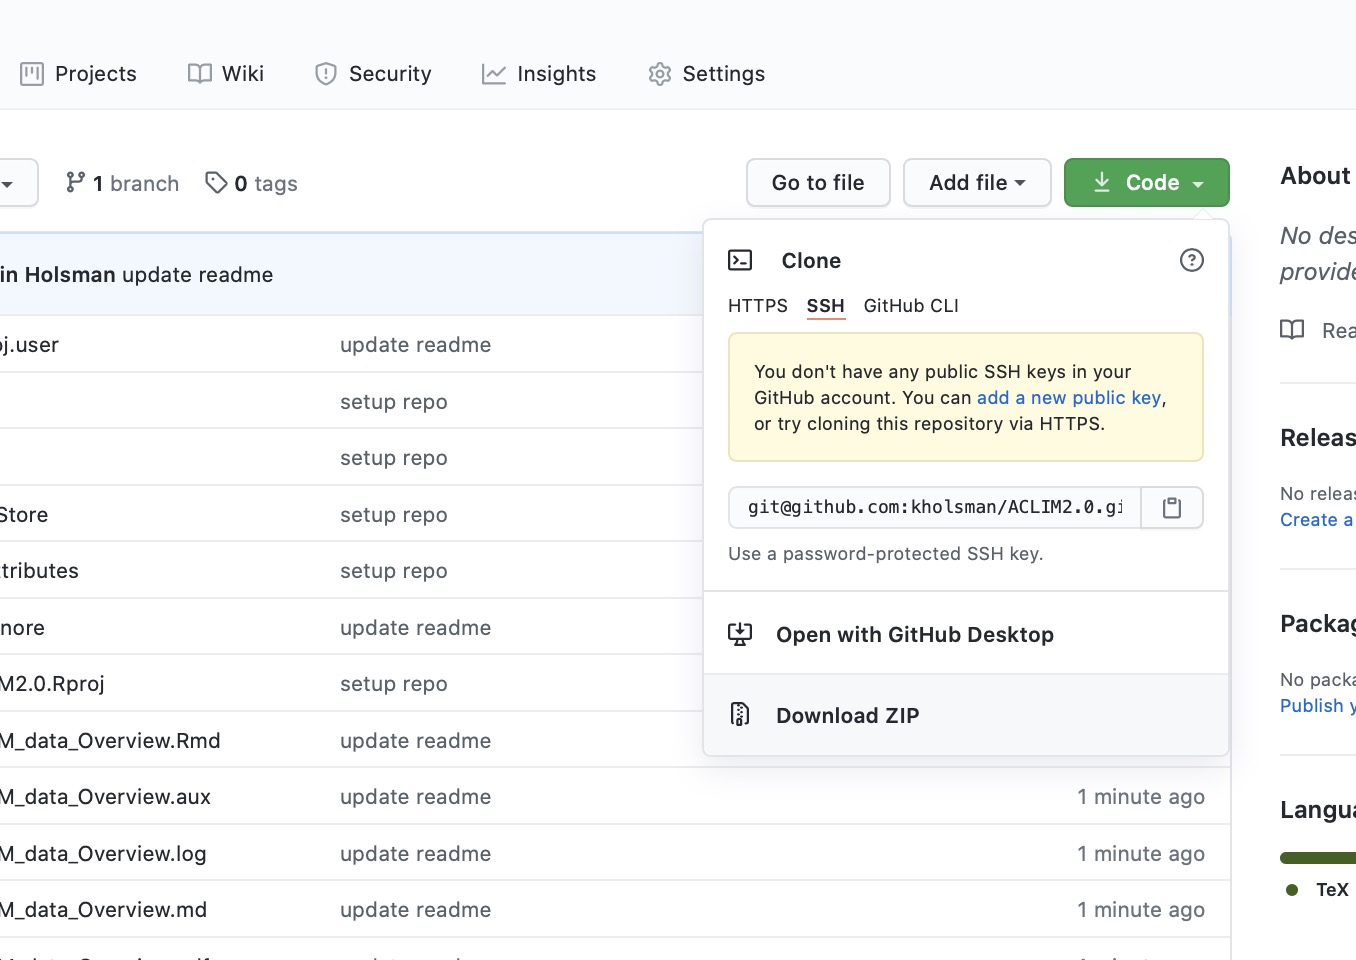
\includegraphics[width=0.4\textwidth,height=\textheight]{Figs/clone.jpg}

\hypertarget{step-2-download-the-data-from-aclim-google-drive}{%
\subsection{2.2. Step 2: Download the data from ACLIM google
drive:}\label{step-2-download-the-data-from-aclim-google-drive}}

Data files are too large to store in the GitHub repository and are
instead saved in the shared ACLIM data folder. For most applications you
can use the ACLIM level3 post-processed indices available on the shared
ACLIM drive in the root google drive data folder:
\href{https://drive.google.com/drive/u/0/folders/0Bx7wdZllbuF9eDJndkhCS2EwQUk}{\textbf{00\_ACLIM\_shared\textgreater02\_DATA}}.

There are two folders that need to be copied into the ACLIM2 folder on
your computer under
`\texttt{\textasciitilde{}{[}YOURPATH{]}/ACLIM2/Data/in/}:

\begin{enumerate}
\def\labelenumi{\arabic{enumi})}
\item
  \href{https://drive.google.com/drive/u/0/folders/0Bx7wdZllbuF9eDJndkhCS2EwQUk}{\textbf{00\_ACLIM\_shared\textgreater02\_DATA\textgreater Newest}}.
  This folder contains a folder called \texttt{roms\_for\_aclim} with
  all the ACLIM Level3 indices for model simulations available to ACLIM
  members.
\item
  \href{https://drive.google.com/drive/u/0/folders/0Bx7wdZllbuF9eDJndkhCS2EwQUk}{\textbf{00\_ACLIM\_shared\textgreater02\_DATA\textgreater Map\_layers.zip}}.
  This file needs to be unzipped after you download it to your local
  folder. It contains (large) base maps for the code below including
  \texttt{shp\_files} and \texttt{geo\_tif} folders.
\end{enumerate}

\begin{figure}
\centering
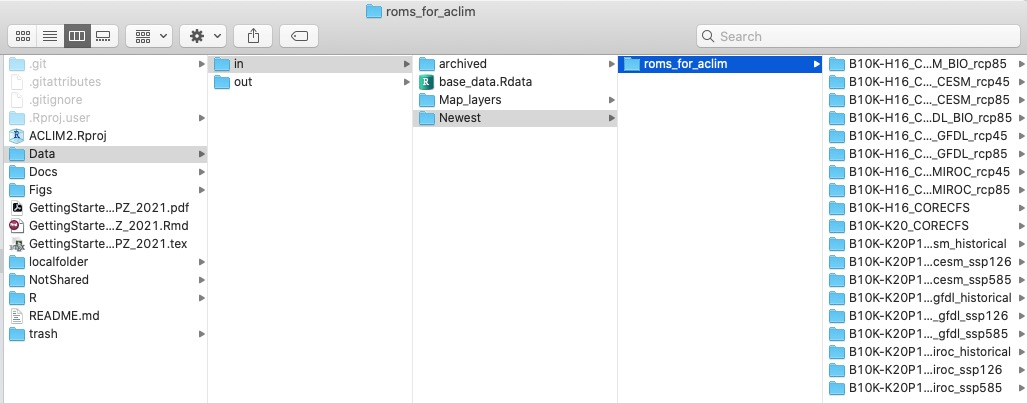
\includegraphics[width=0.65\textwidth,height=\textheight]{Figs/data_dir.jpg}
\caption{Your local \texttt{ACLIM2/Data} directory should look something
like this when you are done downloading the data and unzipping it.}
\end{figure}

\hypertarget{information-about-aclim-level3-indices}{%
\subsection{2.3 Information about ACLIM Level3
indices}\label{information-about-aclim-level3-indices}}

Please be sure to coordinate with ROMSNPZ modeling team members to
ensure data is applied appropriately. If you need access to the raw
ROMSNPZ files (netcdf, non-regridded large files located on MOX). Please
contact \href{albert.j.hermann@noaa.gov}{\textbf{Al Hermann}} or
\href{kelly.kearney@noaa.gov}{\textbf{Kelly Kearney}}.

\textbf{IMPORTANT}\\
The ACLIM indices are stored as netcdf files (.nc) format in the Data
folder of the ACLIM shared google drive. Please note that while the
CMIP5 set is now public (Hermann et al.~2019) \textbf{the CMIP6 suite is
under embargo for QAQC and should not be shared outside of the ACLIM
group}. Al, Wei, Kelly, Darren, and Kerim are in the process of
synthesizing and publishing the CMIP6 data (goal is spring 2021 for
submission), following those publications the data will be made
accessible to the public via the PMEL data portal, as is the case for
the CMIP5 data and public hindcasts. It is strongly recommended that you
include at least one (ideally multiple) authors from the ROMSNPZ team as
co-author on your paper if you are linking to this data, this is
especially the case for the CMIP6 data. There are multiple spatial and
temporal caveats that are best described in discussions with the authors
of these data and inclusion as co-authors will facilitate appropriate
application and interpretation of the ROMSNPZ data.

These files can be used to generate seasonal, monthly, and annual
indices (like those reported in Reum et al.~2020, Holsman et al.~2020).
The \texttt{Newest} folder is organized by Bering10K version, General
Circulation Model (GCM) and carbon scenario,
e.g.~\texttt{B10K-H16\_CMIP5\_CESM\_rcp45}. Within each folder the
following subfolders are:

\begin{itemize}
\tightlist
\item
  \texttt{Level1}: (Empty; not copied from Mox)
\item
  \texttt{Level2}: (Empty; not copied from Mox)
\item
  \texttt{Level3}: 2 files (\texttt{ACLIMsurveyrep\_B10K-x.nc} and
  \texttt{ACLIMregion\_B10K-x.nc} )
\end{itemize}

\begin{enumerate}
\def\labelenumi{\arabic{enumi})}
\tightlist
\item
  \texttt{ACLIMsurveyrep\_B10K-x.nc} contains summer groundfish trawl
  ``survey replicated'' indices (using mean date and lat lon)
  \emph{(Note that the resampling stations need to be removed before
  creating bottom temperature maps)}\\
\item
  \texttt{ACLIMregion\_B10K-x.nc}: contains weekly ``strata'' values
  \emph{(Note that area weighting should be used to combine values
  across multiple strata)}
\end{enumerate}

In section 2 below we explore these indices in more detail using R,
including using (2) above to generate weekly, monthly, and seasonal
indices (e.g.~Fall Zooplankton) for use in biological models.

\hypertarget{coming-soon-pmel-public-web-based-database-beta-testing-phase-currently-limited-to-cmip5}{%
\subsection{2.4. (Coming soon) PMEL public web-based database
(beta-testing phase; currently limited to
CMIP5)}\label{coming-soon-pmel-public-web-based-database-beta-testing-phase-currently-limited-to-cmip5}}

The ROMSNPZ team has been working with
\href{roland.schweitzer@noaa.gov}{Roland Schweitzer} and
\href{peggy.sullivan@noaa.gov}{Peggy Sullivan} to develop the ACLIM Live
Access Server (LAS) to publicly host the published CMIP5 hindcasts and
downscaled projections. This server is in beta testing phase and can be
accessed at the following links:

\hypertarget{las-custom-romsnpz-data-query-mapping-and-plotting-tool}{%
\subsubsection{\texorpdfstring{\href{https://data.pmel.noaa.gov/aclim/las/}{LAS
custom ROMSNPZ data query, mapping, and plotting
tool}}{LAS custom ROMSNPZ data query, mapping, and plotting tool}}\label{las-custom-romsnpz-data-query-mapping-and-plotting-tool}}

\hypertarget{thredds-aclim-data-access-tool}{%
\subsubsection{\texorpdfstring{\href{https://data.pmel.noaa.gov/aclim/thredds/}{THREDDS
ACLIM data access
tool}}{THREDDS ACLIM data access tool}}\label{thredds-aclim-data-access-tool}}

\hypertarget{erdapp-aclim-data-access-tool}{%
\subsubsection{\texorpdfstring{\href{https://data.pmel.noaa.gov/aclim/erddap/}{ERDAPP
ACLIM data access
tool}}{ERDAPP ACLIM data access tool}}\label{erdapp-aclim-data-access-tool}}

\hypertarget{exploring-the-aclim-indices}{%
\section{3. Exploring the ACLIM
indices}\label{exploring-the-aclim-indices}}

The following examples show how to access and plot the ACLIM indices
from their stored netcdf (.nc) format in the Data folder of the ACLIM
shared google drive. Please note that while the CMIP5 set is now public
(Hermann et al.~2019) \textbf{the CMIP6 suite is under embargo for QAQC
and should not be shared outside of the ACLIM group}. Al, Wei, Kelly,
Darren, and Kerim are in the process of synthesizing and publishing the
CMIP6 data (goal is spring 2021 for submission), following those
publications the data will be made accessible to the public via the PMEL
data portal, as is the case for the CMIP5 data and public hindcasts. It
is strongly recommended that you include at least one (ideally multiple)
authors from the ROMSNPZ team as co-author on your paper if you are
linking to this data, this is especially the case for the CMIP6 data.
There are multiple spatial and temporal caveats that are best described
in discussions with the authors of these data and inclusion as
co-authors will facilitate appropriate application and interpretation of
the ROMSNPZ data.

The naming convention of the folders is:
\texttt{B10K-{[}ROMSNPZ\ version{]}\_{[}CMIP{]}\_{[}GCM{]}\_{[}carbon\ scenario{]}}.For
example, the CMIP5 set of indices was downscaled using the H16 (Hermann
et al.~2016) version of the ROMSNPZ. Three models were used to force
boundary conditions( MIROC, CESM, and GFDL) under 2 carbon scenarios RCP
8.5 and RCP 4.5. So to see an individual trajectory we might look in the
level3 (timeseries indices) folder under
\texttt{B10K-H16\_CMIP5\_CESM\_rcp45}, which would be the B10K version
H16 of the CMIP5 CESM model under RCP4.5.

\hypertarget{set-up-the-r-workspace-and-explore-the-two-aclim-level3-indices-types}{%
\subsection{3.1. Set up the R Workspace and explore the two ACLIM Level3
indices
types:}\label{set-up-the-r-workspace-and-explore-the-two-aclim-level3-indices-types}}

The following \texttt{make.R} script will load the directory paths,
preferences, packages, and based functions into R().

\begin{Shaded}
\begin{Highlighting}[]
\NormalTok{    tmstp  <-}\StringTok{ }\KeywordTok{format}\NormalTok{(}\KeywordTok{Sys.time}\NormalTok{(), }\StringTok{"%Y_%m_%d"}\NormalTok{)}
\NormalTok{    main   <-}\StringTok{ }\KeywordTok{getwd}\NormalTok{()  }\CommentTok{#"~/GitHub_new/ACLIM2"}
    
    \CommentTok{# loads packages, data, setup, etc.}
    \KeywordTok{source}\NormalTok{(}\StringTok{"R/make.R"}\NormalTok{)}
\end{Highlighting}
\end{Shaded}

Once the base files and setup are loaded you can explore the index
types. Recall that in each scenario folder there are two indices saved
within the \texttt{Level3} subfolders:

\begin{enumerate}
\def\labelenumi{\arabic{enumi})}
\tightlist
\item
  \texttt{ACLIMsurveyrep\_B10K-x.nc} contains summer groundfish trawl
  ``survey replicated'' indices (using mean date and lat lon)
  \emph{(Note that the resampling stations need to be removed before
  creating bottom temperature maps)}\\
\item
  \texttt{ACLIMregion\_B10K-x.nc}: contains weekly ``strata'' values
  \emph{(Note that area weighting should be used to combine values
  across multiple strata)}
\end{enumerate}

\begin{Shaded}
\begin{Highlighting}[]
    \CommentTok{# list of the scenario x GCM downscaled ACLIM indices}
    \ControlFlowTok{for}\NormalTok{(k }\ControlFlowTok{in}\NormalTok{ aclim)}
     \KeywordTok{cat}\NormalTok{(}\KeywordTok{paste}\NormalTok{(k,}\StringTok{"}\CharTok{\textbackslash{}n}\StringTok{"}\NormalTok{))}
  
    \CommentTok{# get some info about a scenario:}
  
\NormalTok{    all_info1 <-}\StringTok{ }\KeywordTok{info}\NormalTok{(}\DataTypeTok{model_list=}\NormalTok{aclim,}\DataTypeTok{type=}\DecValTok{1}\NormalTok{)}
\NormalTok{    all_info2 <-}\StringTok{ }\KeywordTok{info}\NormalTok{(}\DataTypeTok{model_list=}\NormalTok{aclim,}\DataTypeTok{type=}\DecValTok{2}\NormalTok{)}
\NormalTok{    all_info1}
\NormalTok{    all_info2}
   
    \CommentTok{# variables in each of the two files:}
\NormalTok{    srvy_vars}
\NormalTok{    weekly_vars}
  
    \CommentTok{#summary tables for variables}
\NormalTok{    srvy_var_def}
\NormalTok{    weekly_var_def}
\end{Highlighting}
\end{Shaded}

\hypertarget{explore-survey-replicated-.nc-files-in-r}{%
\subsection{\texorpdfstring{3.2. Explore ``survey replicated''
\texttt{.nc} files in
R()}{3.2. Explore ``survey replicated'' .nc files in R()}}\label{explore-survey-replicated-.nc-files-in-r}}

With the workspace setup the following code can be used to explore the
ACLIM indices.The first indices we will explore are the survey
replicated values for each variable. These are stored in the
\texttt{ACLIMsurveyrep\_B10K-{[}version\_CMIPx\_GCM\_RCP{]}.nc} in each
scenario folder.

\begin{figure}
\centering
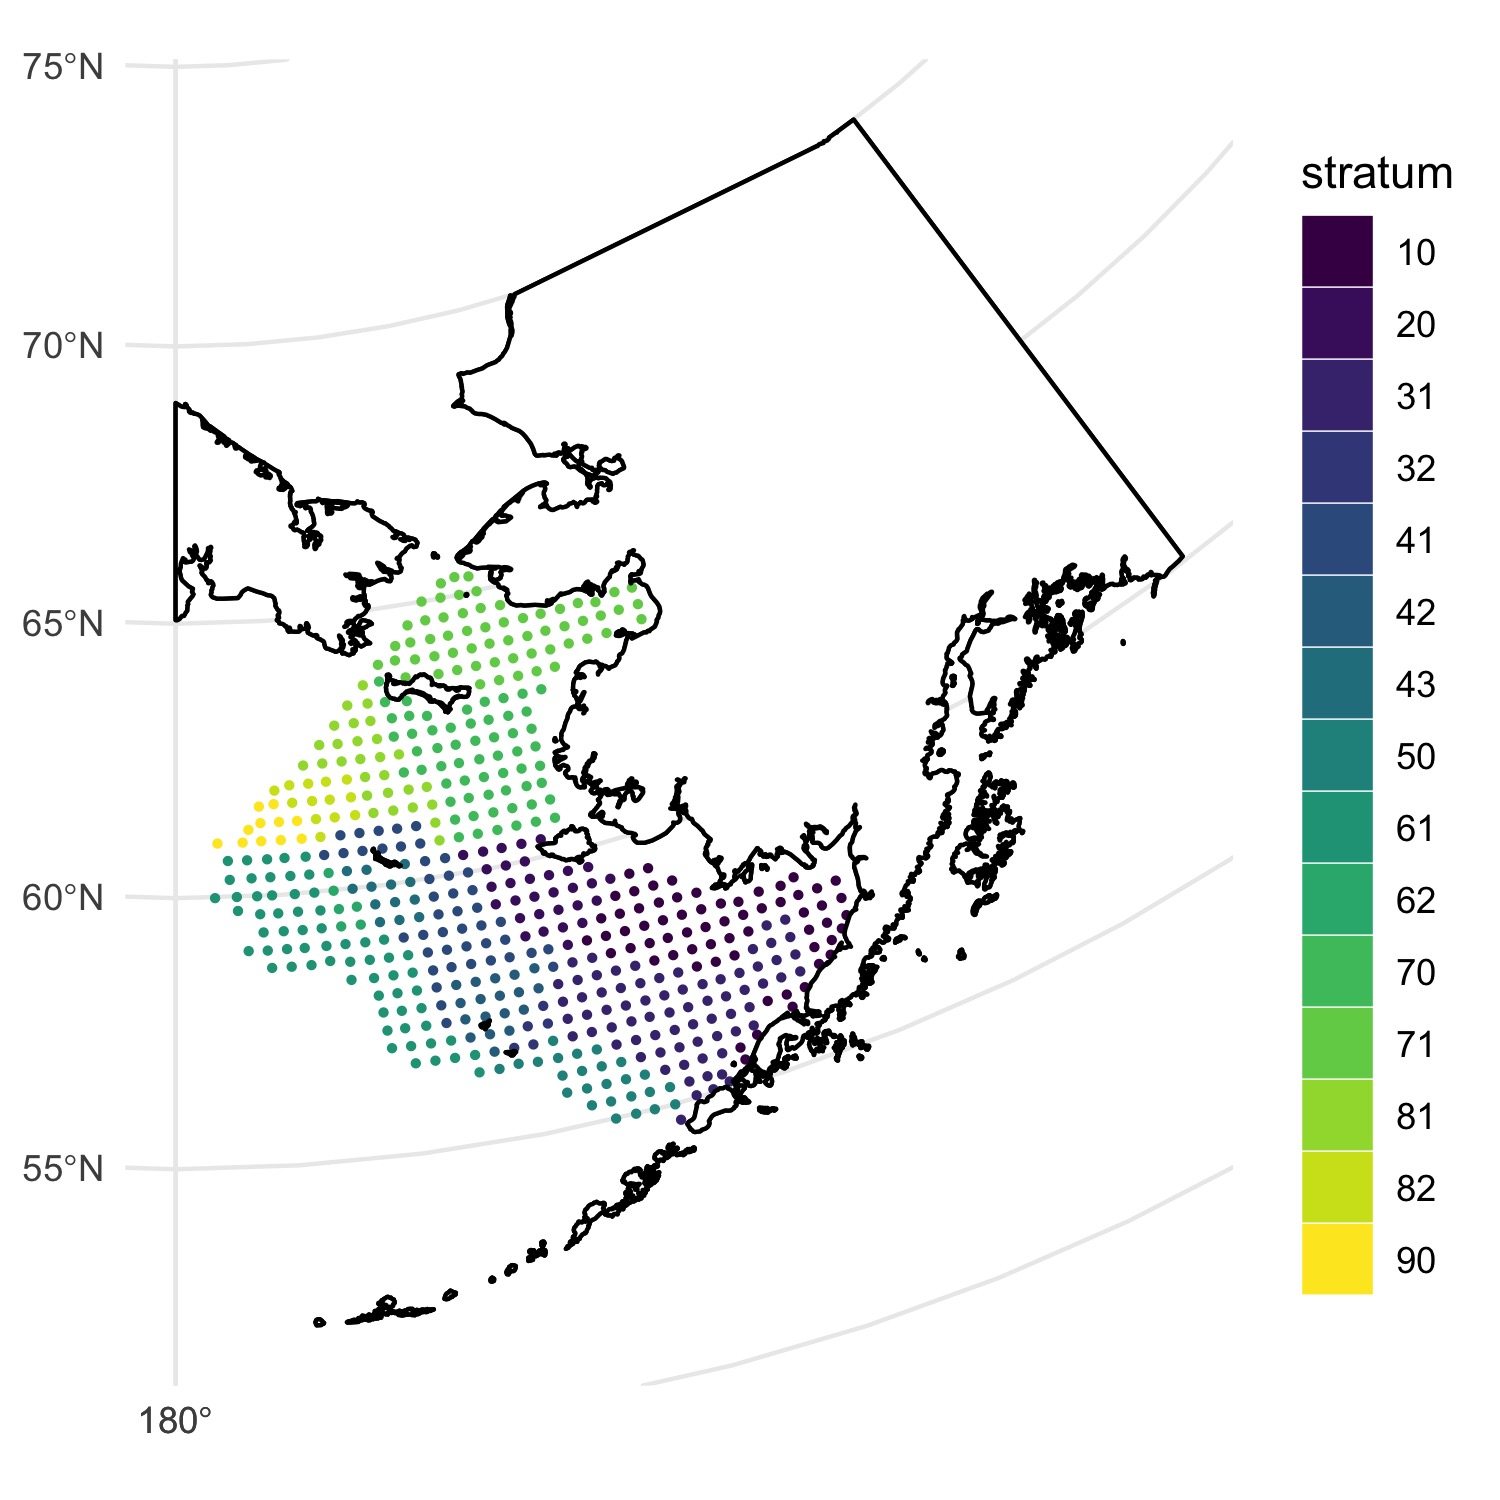
\includegraphics[width=0.3\textwidth,height=\textheight]{Figs/stations.jpg}
\caption{Survey replicated stations.}
\end{figure}

The code segment below will recreate the above figure 2.

\begin{Shaded}
\begin{Highlighting}[]
   \CommentTok{# explore stations in the survey replicated data:}
\NormalTok{   station_info}
  
   \CommentTok{# first convert the station_info object into a shapefile for mapping:}
\NormalTok{   station_sf         <-}\StringTok{ }\KeywordTok{convert2shp}\NormalTok{(station_info)}
\NormalTok{   station_sf}\OperatorTok{$}\NormalTok{stratum <-}\StringTok{ }\KeywordTok{factor}\NormalTok{(station_sf}\OperatorTok{$}\NormalTok{stratum)}
   
   \CommentTok{# plot the stations:}
\NormalTok{   p <-}\StringTok{ }\KeywordTok{plot_stations_basemap}\NormalTok{(}\DataTypeTok{sfIN =}\NormalTok{ station_sf,}\DataTypeTok{fillIN =} \StringTok{"subregion"}\NormalTok{,}\DataTypeTok{colorIN =} \StringTok{"subregion"}\NormalTok{) }\OperatorTok{+}\StringTok{ }
\StringTok{     }\KeywordTok{scale_color_viridis_d}\NormalTok{(}\DataTypeTok{begin =} \FloatTok{.4}\NormalTok{,}\DataTypeTok{end=}\NormalTok{.}\DecValTok{6}\NormalTok{) }\OperatorTok{+}
\StringTok{     }\KeywordTok{scale_fill_viridis_d}\NormalTok{(}\DataTypeTok{begin =} \FloatTok{.4}\NormalTok{,}\DataTypeTok{end=}\NormalTok{.}\DecValTok{6}\NormalTok{)}
\NormalTok{   p}
   
\NormalTok{   p2 <-}\StringTok{ }\KeywordTok{plot_stations_basemap}\NormalTok{(}\DataTypeTok{sfIN =}\NormalTok{ station_sf,}\DataTypeTok{fillIN =} \StringTok{"stratum"}\NormalTok{,}\DataTypeTok{colorIN =} \StringTok{"stratum"}\NormalTok{) }\OperatorTok{+}\StringTok{ }
\StringTok{     }\KeywordTok{scale_color_viridis_d}\NormalTok{() }\OperatorTok{+}
\StringTok{     }\KeywordTok{scale_fill_viridis_d}\NormalTok{()}
\NormalTok{   p2}
   
   \ControlFlowTok{if}\NormalTok{(update.figs)  }\KeywordTok{ggsave}\NormalTok{(}\DataTypeTok{file=}\StringTok{"Figs/stations.jpg"}\NormalTok{,}\DataTypeTok{width=}\DecValTok{5}\NormalTok{,}\DataTypeTok{height=}\DecValTok{5}\NormalTok{)}
\end{Highlighting}
\end{Shaded}

Now let's explore the survey replicated data in more detail and use it
to create a cold pool index for each simulation and hindcast scenario x
model x CMIP combination.

\begin{Shaded}
\begin{Highlighting}[]
    \CommentTok{# now create plots of average BT during four time periods}
\NormalTok{    time_seg   <-}\StringTok{ }\KeywordTok{list}\NormalTok{(}\StringTok{'2010-2020'}\NormalTok{ =}\StringTok{ }\KeywordTok{c}\NormalTok{(}\DecValTok{2010}\OperatorTok{:}\DecValTok{2020}\NormalTok{),}
                        \StringTok{'2021-2040'}\NormalTok{ =}\StringTok{ }\KeywordTok{c}\NormalTok{(}\DecValTok{2021}\OperatorTok{:}\DecValTok{2040}\NormalTok{),}
                        \StringTok{'2041-2060'}\NormalTok{ =}\StringTok{ }\KeywordTok{c}\NormalTok{(}\DecValTok{2041}\OperatorTok{:}\DecValTok{2060}\NormalTok{),}
                        \StringTok{'2061-2080'}\NormalTok{ =}\StringTok{ }\KeywordTok{c}\NormalTok{(}\DecValTok{2061}\OperatorTok{:}\DecValTok{2080}\NormalTok{),}
                        \StringTok{'2081-2099'}\NormalTok{ =}\StringTok{ }\KeywordTok{c}\NormalTok{(}\DecValTok{2081}\OperatorTok{:}\DecValTok{2099}\NormalTok{))}
  
    \CommentTok{# View an individual variable (e.g., Bottom Temp)}
    \CommentTok{# -------------------------------------------------------}
\NormalTok{    srvy_vars}
\NormalTok{    aclim}
\NormalTok{    sim <-}\StringTok{ }\NormalTok{aclim[}\DecValTok{2}\NormalTok{]}
    \CommentTok{# open a "region" or strata specific nc file}
\NormalTok{    ncfl      <-}\StringTok{ }\KeywordTok{file.path}\NormalTok{(sim,}\KeywordTok{paste0}\NormalTok{(srvy_txt,sim,}\StringTok{".nc"}\NormalTok{))}
\NormalTok{    nc        <-}\StringTok{ }\KeywordTok{nc_open}\NormalTok{(}\KeywordTok{file.path}\NormalTok{(data_path,ncfl))}
    
    \CommentTok{# convert the nc files into a data.frame}
\NormalTok{    tmp_var    <-}\StringTok{ }\KeywordTok{convert2df}\NormalTok{(}\DataTypeTok{ncIN =}\NormalTok{ nc, }\DataTypeTok{type =} \DecValTok{2}\NormalTok{, }\DataTypeTok{varIN =} \StringTok{"temp_bottom5m"}\NormalTok{)}
    \KeywordTok{head}\NormalTok{(tmp_var)}
    \KeywordTok{nc_close}\NormalTok{(nc)}
    
    
    \CommentTok{# Collate mean values across timeperiods and simulations}
    \CommentTok{# -------------------------------------------------------}
\NormalTok{    m_set      <-}\StringTok{ }\KeywordTok{c}\NormalTok{(}\DecValTok{18}\NormalTok{,}\DecValTok{19}\NormalTok{);aclim[m_set]}
\NormalTok{    mn_var_all <-}\StringTok{ }\KeywordTok{get_mn_srvy_var}\NormalTok{(}\DataTypeTok{modset =}\NormalTok{ aclim[m_set],}\DataTypeTok{varUSE=}\StringTok{"temp_bottom5m"}\NormalTok{)}
\NormalTok{    mn_var_sf  <-}\StringTok{ }\KeywordTok{convert2shp}\NormalTok{(mn_var_all}\OperatorTok\KeywordTok{filter}\NormalTok{(}\OperatorTok{!}\KeywordTok{is.na}\NormalTok{(mnval)))}
   
\NormalTok{    p3         <-}\StringTok{ }\KeywordTok{plot_stations_basemap}\NormalTok{(}\DataTypeTok{sfIN =}\NormalTok{ mn_var_sf,}
                                \DataTypeTok{fillIN =} \StringTok{"mnval"}\NormalTok{,}
                                \DataTypeTok{colorIN =} \StringTok{"mnval"}\NormalTok{,}
                                \DataTypeTok{sizeIN=}\NormalTok{.}\DecValTok{3}\NormalTok{) }\OperatorTok{+}
\StringTok{      }\KeywordTok{facet_grid}\NormalTok{(simulation}\OperatorTok{~}\NormalTok{time_period)}\OperatorTok{+}
\StringTok{      }\KeywordTok{scale_color_viridis_c}\NormalTok{()}\OperatorTok{+}
\StringTok{      }\KeywordTok{scale_fill_viridis_c}\NormalTok{()}\OperatorTok{+}
\StringTok{      }\KeywordTok{guides}\NormalTok{(}
        \DataTypeTok{color =}  \KeywordTok{guide_legend}\NormalTok{(}\DataTypeTok{title=}\StringTok{"Bottom T (degC)"}\NormalTok{),}
        \DataTypeTok{fill  =}  \KeywordTok{guide_legend}\NormalTok{(}\DataTypeTok{title=}\StringTok{"Bottom T (degC)"}\NormalTok{)) }\OperatorTok{+}
\StringTok{      }\KeywordTok{ggtitle}\NormalTok{(}\KeywordTok{substr}\NormalTok{(aclim[m_set[}\DecValTok{1}\NormalTok{]],}\DecValTok{1}\NormalTok{,}\DecValTok{23}\NormalTok{))}
   
    \CommentTok{# This is slow but it works (repeat dev.new() twice if in Rstudio)...}
    \KeywordTok{dev.new}\NormalTok{()}
\NormalTok{    p3}
    
    \ControlFlowTok{if}\NormalTok{(update.figs)  }\KeywordTok{ggsave}\NormalTok{(}\DataTypeTok{file=}\StringTok{"Figs/mn_BT.jpg"}\NormalTok{,}\DataTypeTok{width=}\DecValTok{8}\NormalTok{,}\DataTypeTok{height=}\DecValTok{5}\NormalTok{)}
  
    \KeywordTok{graphics.off}\NormalTok{()}
\end{Highlighting}
\end{Shaded}

\begin{figure}
\centering
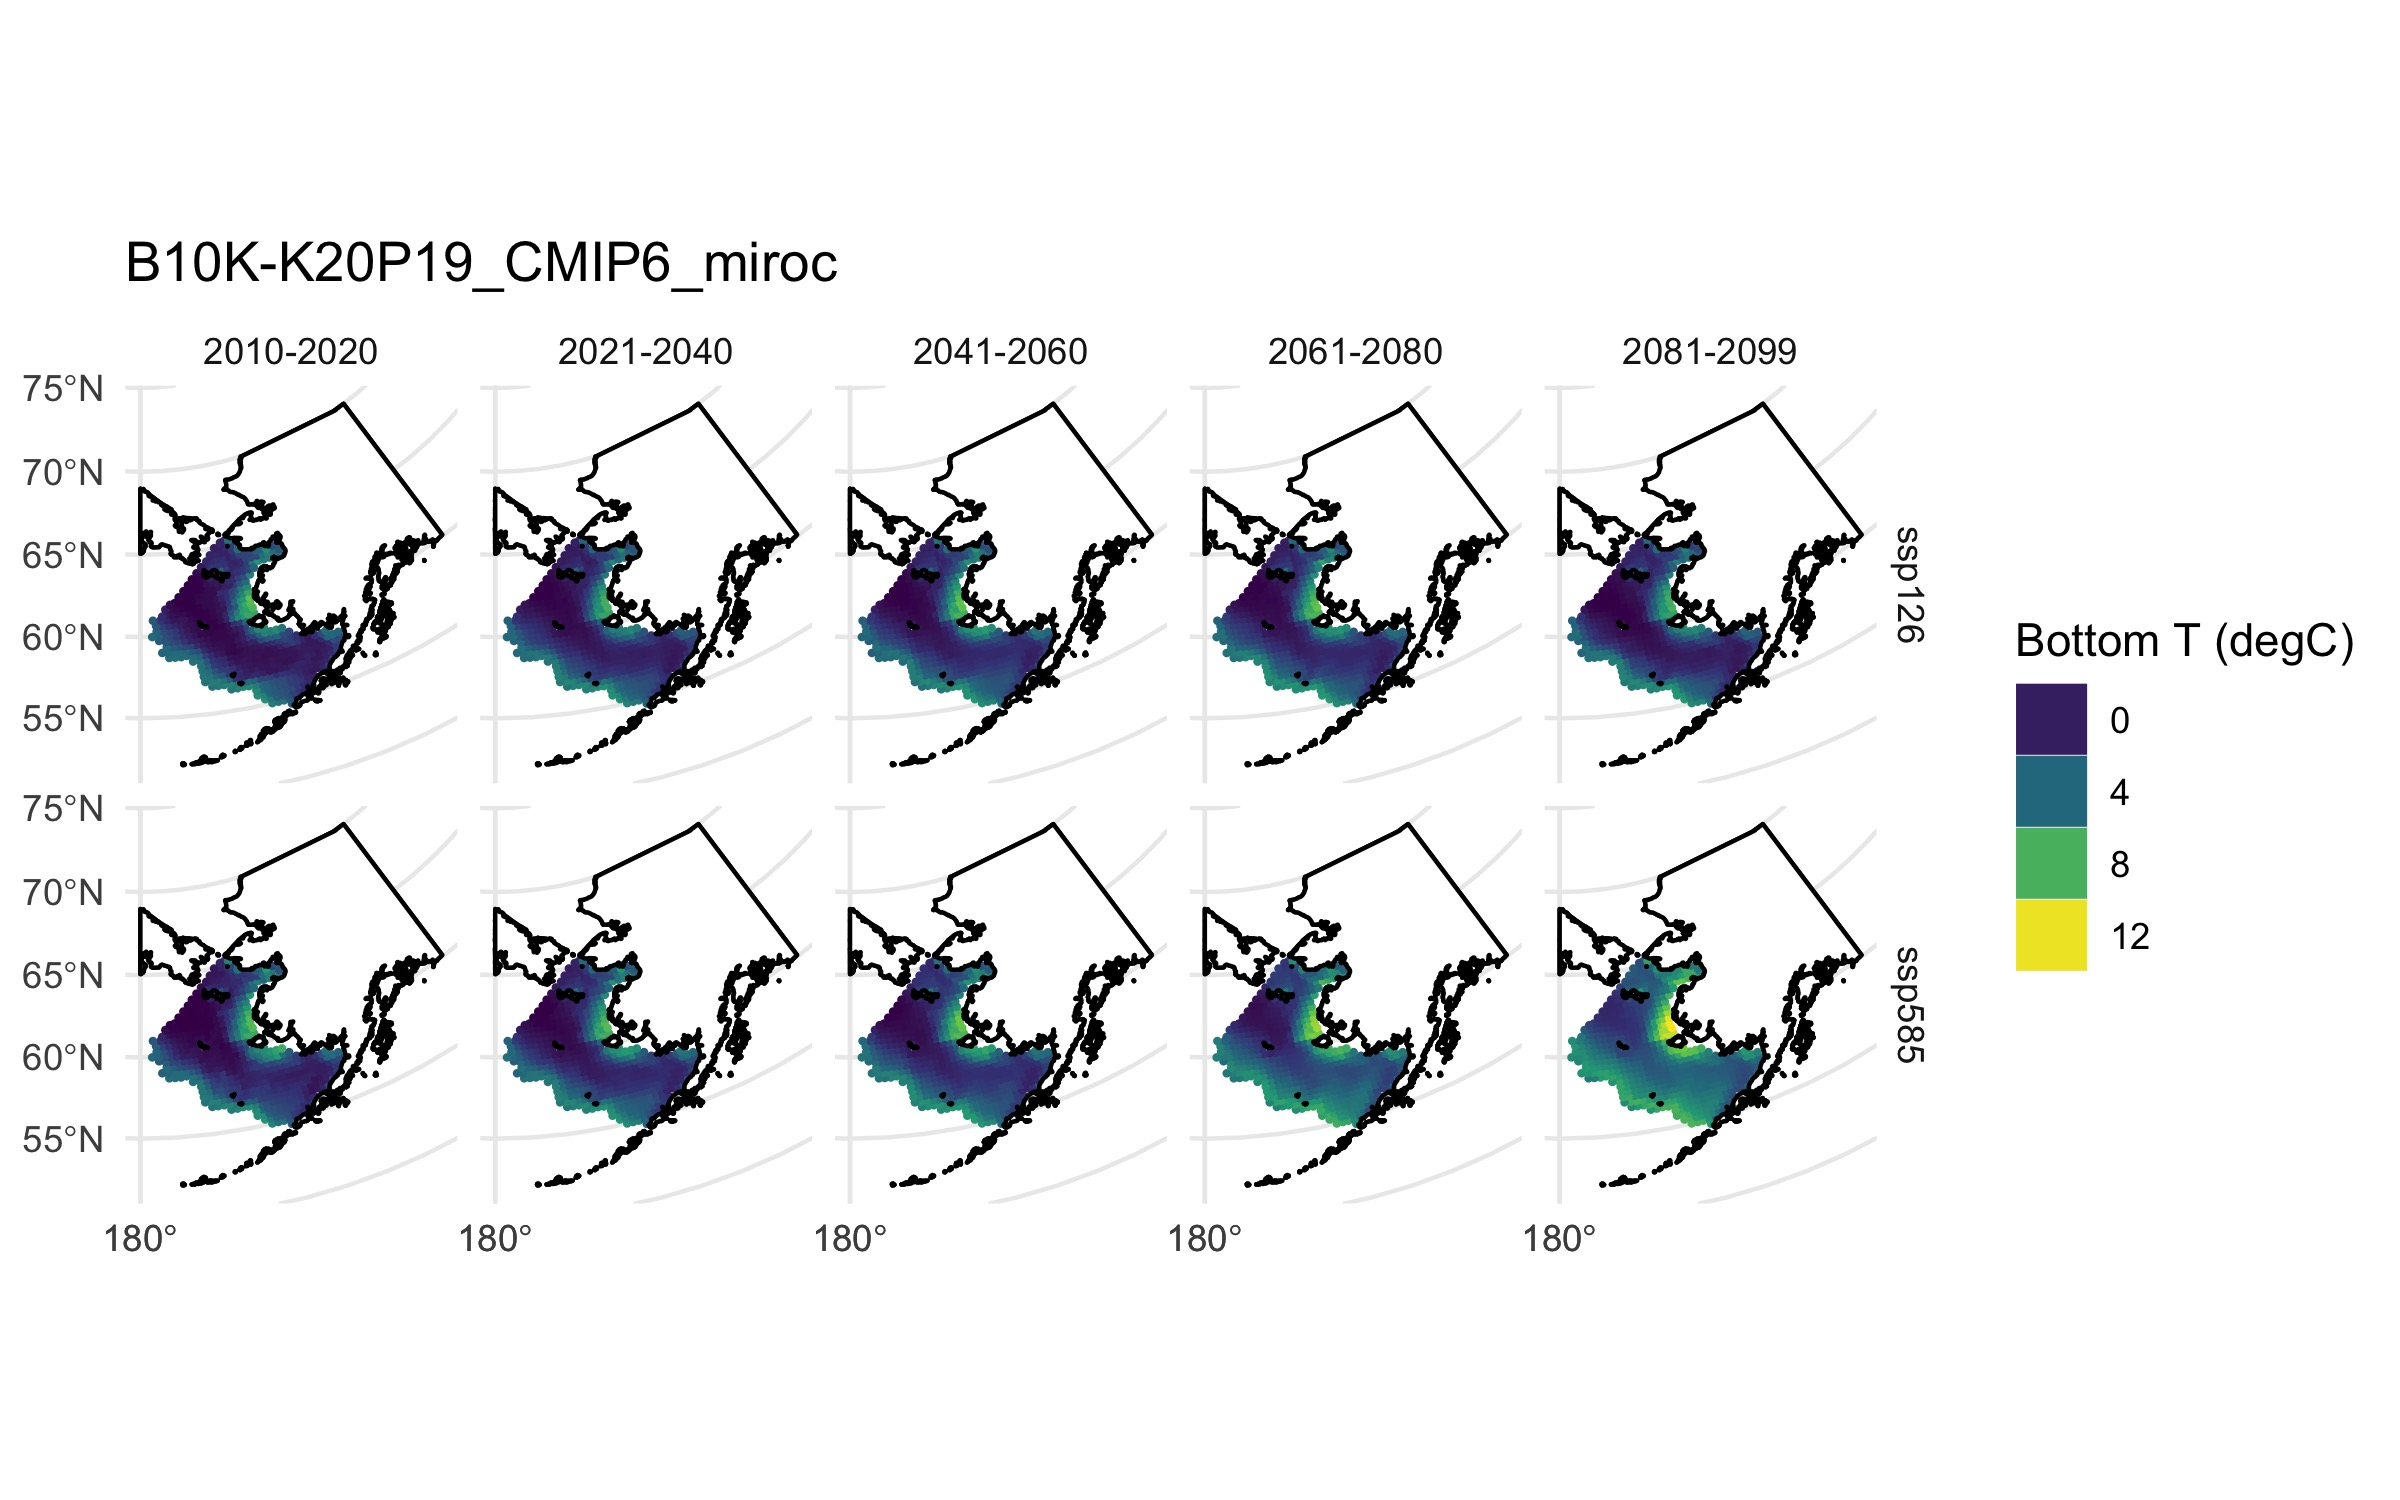
\includegraphics{Figs/mn_BT.jpg}
\caption{Bottom temperature projections under differing SSP126 (top row)
and SSP585 (bottom row)}
\end{figure}

\hypertarget{explore-weekly-strata-.nc-files-in-r}{%
\subsection{\texorpdfstring{3.3. Explore ``weekly strata'' \texttt{.nc}
files in
R()}{3.3. Explore ``weekly strata'' .nc files in R()}}\label{explore-weekly-strata-.nc-files-in-r}}

The next set of indices to will explore are the weekly strata-specific
values for each variable.These are stored in the
\texttt{ACLIMregion\_B10K-{[}version\_CMIPx\_GCM\_RCP{]}.nc} in each
scenario folder.

\begin{Shaded}
\begin{Highlighting}[]
    \CommentTok{# list of the scenario x GCM downscaled ACLIM indices}
    \ControlFlowTok{for}\NormalTok{(k }\ControlFlowTok{in}\NormalTok{ aclim)}
      \KeywordTok{cat}\NormalTok{(}\KeywordTok{paste}\NormalTok{(k,}\StringTok{"}\CharTok{\textbackslash{}n}\StringTok{"}\NormalTok{)}

    \CommentTok{# View an individual variable (e.g., Bottom Temp)}
    \CommentTok{# -------------------------------------------------------}
\NormalTok{    weekly_vars}
\NormalTok{    aclim}
\NormalTok{    sim <-}\StringTok{ }\NormalTok{aclim[}\DecValTok{2}\NormalTok{]}
    \CommentTok{# open a "region" or strata specific nc file}
\NormalTok{    ncfl      <-}\StringTok{ }\KeywordTok{file.path}\NormalTok{(sim,}\KeywordTok{paste0}\NormalTok{(reg_txt,sim,}\StringTok{".nc"}\NormalTok{))}
\NormalTok{    nc        <-}\StringTok{ }\KeywordTok{nc_open}\NormalTok{(}\KeywordTok{file.path}\NormalTok{(data_path,ncfl))}
    
    \CommentTok{# convert the nc files into a data.frame}
\NormalTok{    tmp_var    <-}\StringTok{ }\KeywordTok{convert2df}\NormalTok{(}\DataTypeTok{ncIN =}\NormalTok{ nc, }\DataTypeTok{type =} \DecValTok{1}\NormalTok{, }\DataTypeTok{varIN =} \StringTok{"temp_bottom5m"}\NormalTok{)}
    \KeywordTok{head}\NormalTok{(tmp_var)}
    \KeywordTok{nc_close}\NormalTok{(nc)}
    
  
   \CommentTok{# now plot the data:}
   
\NormalTok{   p4 <-}\StringTok{ }\KeywordTok{ggplot}\NormalTok{(}\DataTypeTok{data =}\NormalTok{ tmp_var) }\OperatorTok{+}\StringTok{ }
\StringTok{     }\KeywordTok{geom_line}\NormalTok{(}\KeywordTok{aes}\NormalTok{(}\DataTypeTok{x=}\NormalTok{time,}\DataTypeTok{y=}\NormalTok{val,}\DataTypeTok{color=}\NormalTok{ strata),}\DataTypeTok{alpha=}\NormalTok{.}\DecValTok{8}\NormalTok{)}\OperatorTok{+}
\StringTok{     }\KeywordTok{facet_grid}\NormalTok{(basin}\OperatorTok{~}\NormalTok{.)}\OperatorTok{+}
\StringTok{     }\KeywordTok{ylab}\NormalTok{(tmp_var}\OperatorTok{$}\NormalTok{units[}\DecValTok{1}\NormalTok{])}\OperatorTok{+}
\StringTok{     }\KeywordTok{ggtitle}\NormalTok{(}\KeywordTok{substr}\NormalTok{( aclim[i],}\DecValTok{18}\NormalTok{,}\KeywordTok{nchar}\NormalTok{( aclim[i])}\OperatorTok{-}\DecValTok{3}\NormalTok{))}\OperatorTok{+}
\StringTok{     }\KeywordTok{theme_minimal}\NormalTok{()}
\NormalTok{   p4}
   
   \CommentTok{# To get the average value for a set of strata, weight the val by the area:}
\NormalTok{   mn_NEBS <-}\StringTok{ }\KeywordTok{getAVGnSUM}\NormalTok{(}\DataTypeTok{strataIN =}\NormalTok{ NEBS_strata, }\DataTypeTok{dataIN =}\NormalTok{ tmp_var)}
\NormalTok{   mn_NEBS}\OperatorTok{$}\DataTypeTok{basin =} \StringTok{"NEBS"}
\NormalTok{   mn_SEBS <-}\KeywordTok{getAVGnSUM}\NormalTok{(}\DataTypeTok{strataIN =}\NormalTok{ SEBS_strata, }\DataTypeTok{dataIN =}\NormalTok{ tmp_var)}
\NormalTok{   mn_SEBS}\OperatorTok{$}\DataTypeTok{basin =} \StringTok{"SEBS"}
   
\NormalTok{   p5 <-}\StringTok{ }\KeywordTok{ggplot}\NormalTok{(}\DataTypeTok{data =} \KeywordTok{rbind}\NormalTok{(mn_NEBS,mn_SEBS)) }\OperatorTok{+}\StringTok{ }
\StringTok{      }\KeywordTok{geom_line}\NormalTok{(}\KeywordTok{aes}\NormalTok{(}\DataTypeTok{x=}\NormalTok{time,}\DataTypeTok{y=}\NormalTok{mn_val,}\DataTypeTok{color=}\NormalTok{basin),}\DataTypeTok{alpha=}\NormalTok{.}\DecValTok{8}\NormalTok{)}\OperatorTok{+}
\StringTok{      }\KeywordTok{geom_smooth}\NormalTok{(}\KeywordTok{aes}\NormalTok{(}\DataTypeTok{x=}\NormalTok{time,}\DataTypeTok{y=}\NormalTok{mn_val,}\DataTypeTok{color=}\NormalTok{basin),}
                  \DataTypeTok{formula =}\NormalTok{ y }\OperatorTok{~}\StringTok{ }\NormalTok{x, }\DataTypeTok{se =}\NormalTok{ T)}\OperatorTok{+}
\StringTok{      }\KeywordTok{facet_grid}\NormalTok{(basin}\OperatorTok{~}\NormalTok{.)}\OperatorTok{+}
\StringTok{      }\KeywordTok{scale_color_viridis_d}\NormalTok{(}\DataTypeTok{begin=}\NormalTok{.}\DecValTok{4}\NormalTok{,}\DataTypeTok{end=}\NormalTok{.}\DecValTok{8}\NormalTok{)}\OperatorTok{+}
\StringTok{      }\KeywordTok{ylab}\NormalTok{(tmp_var}\OperatorTok{$}\NormalTok{units[}\DecValTok{1}\NormalTok{])}\OperatorTok{+}
\StringTok{      }\KeywordTok{ggtitle}\NormalTok{( aclim[}\DecValTok{2}\NormalTok{])}\OperatorTok{+}
\StringTok{      }\KeywordTok{theme_minimal}\NormalTok{()}
\NormalTok{  p5}
  \ControlFlowTok{if}\NormalTok{(update.figs)  }\KeywordTok{ggsave}\NormalTok{(}\DataTypeTok{file=}\StringTok{"Figs/weekly_byreg.jpg"}\NormalTok{,}\DataTypeTok{width=}\DecValTok{8}\NormalTok{,}\DataTypeTok{height=}\DecValTok{5}\NormalTok{)}
\end{Highlighting}
\end{Shaded}

\begin{figure}
\centering
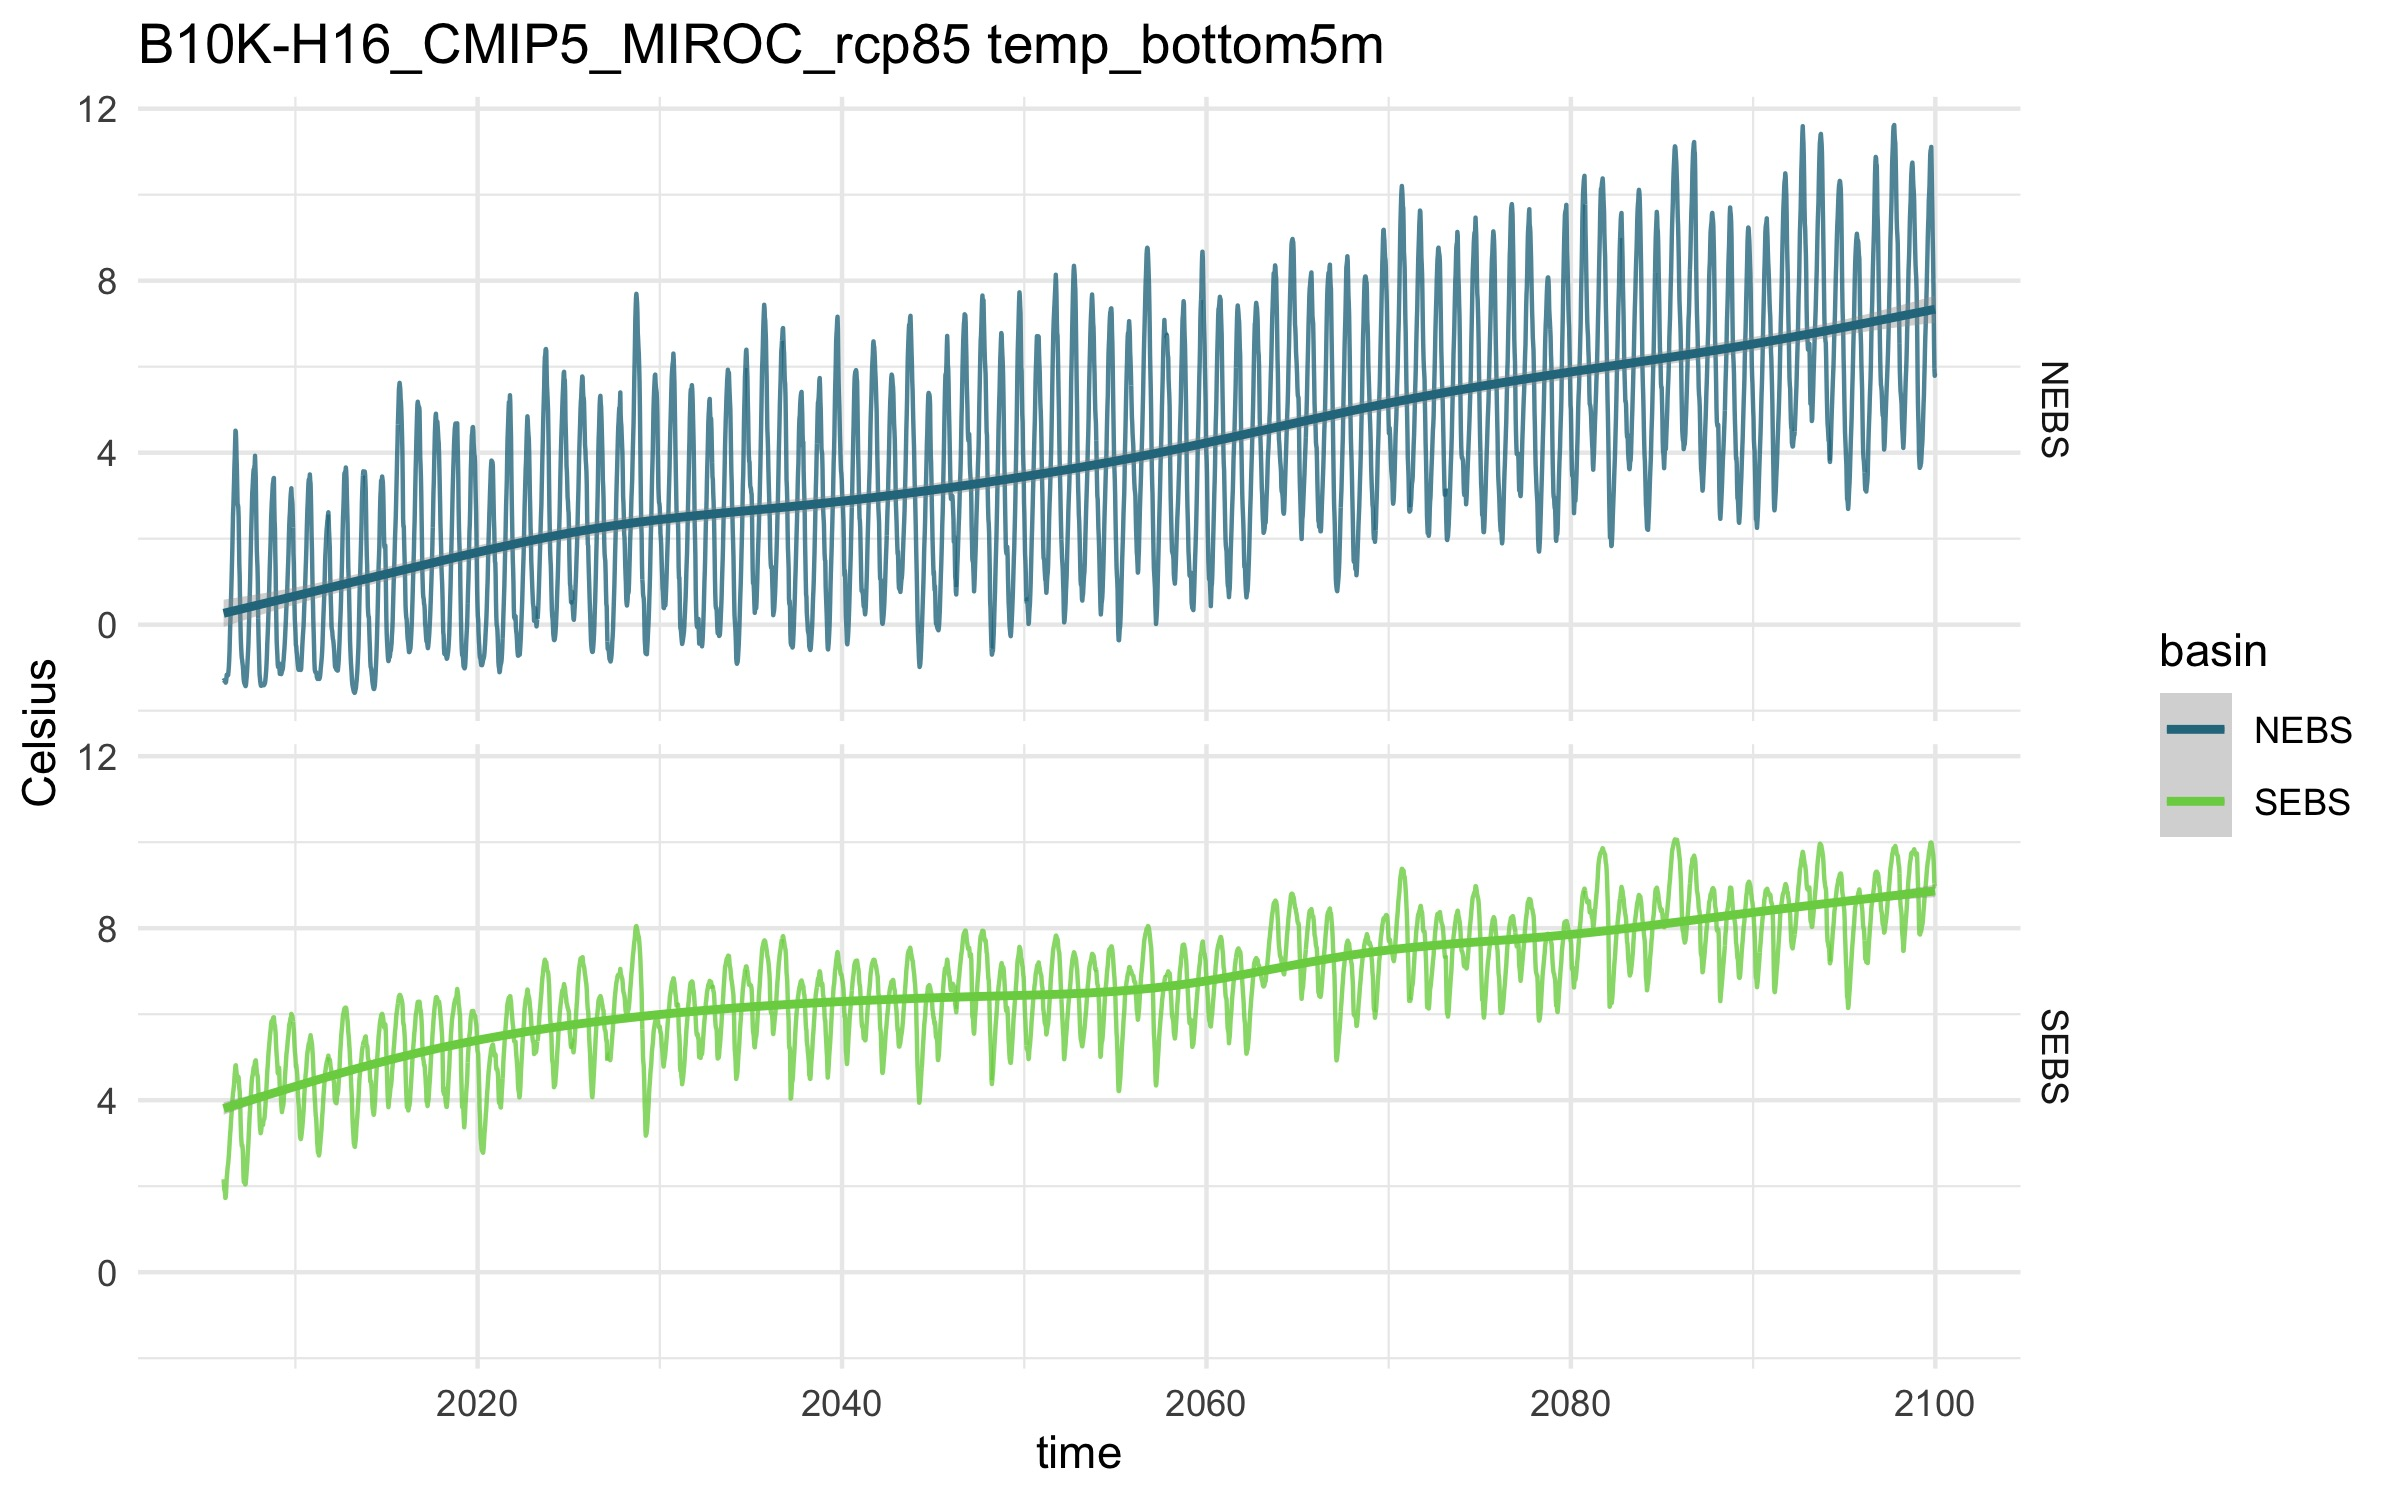
\includegraphics[width=0.65\textwidth,height=\textheight]{Figs/weekly_byreg.jpg}
\caption{Weekly indcices by sub-region}
\end{figure}

\hypertarget{create-monthly-averages}{%
\subsubsection{2.2.4 Create monthly
averages}\label{create-monthly-averages}}

TBA

\hypertarget{create-seasonal-averages}{%
\subsubsection{2.2.5 Create seasonal
averages}\label{create-seasonal-averages}}

TBA

\hypertarget{funding-and-acknowledgments-needs-updating}{%
\section{4. Funding and acknowledgments (needs
updating):}\label{funding-and-acknowledgments-needs-updating}}

\hypertarget{please-include-a-statement-like-the-following-one-in-your-acknowledgements-section}{%
\subsubsection{PLEASE Include a statement like the following one in your
acknowledgements
section:}\label{please-include-a-statement-like-the-following-one-in-your-acknowledgements-section}}

\emph{This study is part of NOAA's Alaska Climate Integrated Modeling
project (ACLIM) and FATE project XXXX. We would like to that the entire
ACLIM team including \texttt{{[}add\ specific\ names{]}} for feedback
and discussions on the broader application of this work. Multiple NOAA
National Marine Fisheries programs provided support for ACLIM including
Fisheries and the Environment (FATE), Stock Assessment Analytical
Methods (SAAM) Science and Technology North Pacific Climate Regimes and
Ecosystem Productivity, the Integrated Ecosystem Assessment Program
(IEA), the NOAA Economics and Social Analysis Division, NOAA Research
Transition Acceleration Program (RTAP), the Alaska Fisheries Science
Center (ASFC), the Office of Oceanic and Atmospheric Research (OAR) and
the National Marine Fisheries Service (NMFS). The scientific views,
opinions, and conclusions expressed herein are solely those of the
authors and do not represent the views, opinions, or conclusions of NOAA
or the Department of Commerce.}

\hypertarget{for-some-of-the-integrated-papers-the-following-maybe-should-also-be-added}{%
\subsubsection{For some of the integrated papers the following maybe
should also be
added:}\label{for-some-of-the-integrated-papers-the-following-maybe-should-also-be-added}}

\emph{Additionally, the International Council for the Exploration of the
Sea (ICES) and the North Pacific Marine Science Organization (PICES)
provided support for Strategic Initiative for the Study of Climate
Impacts on Marine Ecosystems (SI-CCME) workshops, which facilitated
development of the ideas presented in this paper. The scientific views,
opinions, and conclusions expressed herein are solely those of the
authors and do not represent the views, opinions, or conclusions of
NOAA, the Department of Commerce, ICES, or PICES.}

\hypertarget{helpful-links-and-further-reading}{%
\section{5. Helpful links and further
reading:}\label{helpful-links-and-further-reading}}

\hypertarget{citations-for-gcms-and-carbon-scenarios}{%
\subsection{5.1 Citations for GCMs and carbon
scenarios:}\label{citations-for-gcms-and-carbon-scenarios}}

\hypertarget{cmip3-bsierp-global-climate-model-runs}{%
\subsubsection{CMIP3 (BSIERP global climate model
runs):}\label{cmip3-bsierp-global-climate-model-runs}}

Meehl, G. A., C. Covey, T. Delworth, M. Latif, B. McAvaney, J. F. B.
Mitchell, R. J. Stouffer, and K. E. Taylor, 2007: The WCRP CMIP3
multimodel dataset: A new era in climate change research. Bull. Amer.
Meteor. Soc., 88, 1383--1394.

\hypertarget{cmip5-aclim-global-climate-model-runs}{%
\subsubsection{CMIP5 (ACLIM global climate model
runs):}\label{cmip5-aclim-global-climate-model-runs}}

Taylor, K. E., R. J. Stouffer, and G. A. Meehl, 2012:Anoverview of CMIP5
and the experiment design. Bull. Amer. Meteor. Soc., 93, 485--498.

\hypertarget{cmip6-and-ssps-aclim2-global-climate-model-runs}{%
\subsubsection{CMIP6 and SSPs (ACLIM2 global climate model
runs):}\label{cmip6-and-ssps-aclim2-global-climate-model-runs}}

ONeill, B. C., C. Tebaldi, D. P. van Vuuren, V. Eyring, P.
Friedlingstein, G. Hurtt, R. Knutti, E. Kriegler, J.-F. Lamarque, J.
Lowe, G. A. Meehl, R. Moss, K. Riahi, and B. M. Sanderson. 2016. The
Scenario Model Intercomparison Project (ScenarioMIP) for CMIP6.
Geoscientific Model Development 9:3461--3482.

\hypertarget{weblinks-for-further-reading}{%
\subsection{5.2 Weblinks for further
reading:}\label{weblinks-for-further-reading}}

\begin{itemize}
\item
  Explore annual indices of downscaled projections for the EBS:
  \href{https://kholsman.shinyapps.io/aclim/}{\textbf{ACLIM indices}}
\item
  To view climate change projections from CMIP5 (eventually
  CMIP6):\href{https://www.esrl.noaa.gov/psd/ipcc/ocn/}{\textbf{ESRL
  climate change portal }}
\end{itemize}

\hypertarget{additional-information-on-hindcast-and-projection-models-needs-updating}{%
\subsection{5.3 Additional information on Hindcast and Projection Models
(needs
updating)}\label{additional-information-on-hindcast-and-projection-models-needs-updating}}

\hypertarget{core-cfsr-1976-2012}{%
\subsubsection{CORE-CFSR (1976-2012)}\label{core-cfsr-1976-2012}}

This is the hindcast for the Bering Sea and is a combination of the
reconstructed climatology from the
\href{http://portal.aoos.org/bering-sea.php\#module-metadata/5626a0b6-7d79-11e3-ac17-00219bfe5678/0756e6c2-a8e2-40af-aa3d-22051ed68067}{\textbf{CLIVAR}}
Co-ordinated Ocean-Ice Reference Experiments (CORE) Climate Model
(1969-2006) the
\href{http://portal.aoos.org/bering-sea.php\#module-metadata/f8cb79f6-7d59-11e3-a6ee-00219bfe5678/2deb2eca-f3f5-4eda-a132-112468711de7}{\textbf{NCEP}}
Climate Forecast System Reanalysis is a set of re-forecasts carried out
by NOAA's National Center for Environmental Prediction (NCEP). See
\href{http://cfs.ncep.noaa.gov/cfsr/}{\textbf{CFS-R}} for more info.

\hypertarget{cccma2006-2039-ar4-sres-a1b}{%
\subsubsection{\texorpdfstring{\href{http://www.cccma.ec.gc.ca/diagnostics/cgcm3/cgcm3.shtml}{CCCMA}(2006-2039;
AR4 SRES
A1B)}{CCCMA(2006-2039; AR4 SRES A1B)}}\label{cccma2006-2039-ar4-sres-a1b}}

Developed by the Canadian Centre for Climate Modelling and Analysis,
this is also known as the CGCM3/T47 model. This model showed the
greatest warming over time compared to other models tested by PMEL. See
more data the
\href{http://portal.aoos.org/bering-sea.php\#module-metadata/4f706756-7d57-11e3-bce5-00219bfe5678/ffa1bcc1-288d-4f8e-912e-500a618b241a}{\textbf{AOOS:CCCMA
portal}}.

\hypertarget{echog2006-2039-ar4-sres-a1b}{%
\subsubsection{\texorpdfstring{\href{http://www-pcmdi.llnl.gov/ipcc/model_documentation/ECHO-G.pdf}{ECHOG}(2006-2039;
AR4 SRES
A1B)}{ECHOG(2006-2039; AR4 SRES A1B)}}\label{echog2006-2039-ar4-sres-a1b}}

The ECHO-G model from the Max Planck Institute in Germany This model
showed the least warming over time compared to other models tested by
PMEL. See more data the AOOS:ECHO-G portal.

\hypertarget{gfdl-2006-2100-ar5-rcp-4.5-8.5-ssp126ssp585}{%
\subsubsection{\texorpdfstring{\href{http://www.gfdl.noaa.gov/earth-system-model}{GFDL}
(2006-2100; AR5 RCP 4.5, 8.5,
SSP126,SSP585)}{GFDL (2006-2100; AR5 RCP 4.5, 8.5, SSP126,SSP585)}}\label{gfdl-2006-2100-ar5-rcp-4.5-8.5-ssp126ssp585}}

The NOAA Geophysical Fluid Dynamics Laboratory
\href{http://www.gfdl.noaa.gov}{\textbf{GFDL}} has lead development of
the first Earth System Models (ESMs), which like physical climate
models, are based on an atmospheric circulation model coupled with an
oceanic circulation model, with representations of land, sea ice and
iceberg dynamics; ESMs additionally incorporate interactive
biogeochemistry, including the carbon cycle. The ESM2M model used in
this project is an evolution of the prototype EMS2.1 model, where
pressure-based vertical coordinates are used along the developmental
path of GFDL's Modular Ocean Model version 4.1 and where the land model
is more adavanced (LM3) than in the previous ESM2.1

\hypertarget{miroc2006-2039-ar4-sres-a1b-2006-2100-rcp4.5-rcp8.5-ssp585-ssp126}{%
\subsubsection{\texorpdfstring{\href{www.cger.nies.go.jp/publications/report/i073/I073.pdf}{MIROC}(2006-2039;
AR4 SRES A1B; 2006-2100 RCP4.5, RCP8.5, SSP585,
SSP126)}{MIROC(2006-2039; AR4 SRES A1B; 2006-2100 RCP4.5, RCP8.5, SSP585, SSP126)}}\label{miroc2006-2039-ar4-sres-a1b-2006-2100-rcp4.5-rcp8.5-ssp585-ssp126}}

The Model for Interdisciplinary Research on Climate (MIROC)-M model
developed by a consortium of agencies in Japan {[}{]}. Compared to other
models tested by PMEL, MIROC-M was intermediate in degree of warming
over the Bering Sea shelf for the first half of the 21st century. See
more data the AOOS:MIROC portal.

\end{document}
